\chapter{石墨烯的生长机理研究}
\section{引言}
    如今,化学气相沉积法已经成为大规模石墨烯生长的主要合成方法。以铜为代表的金属衬底对含碳前驱体的催化作用极大提升了石墨烯的产率。同时,铜衬底自限制效应及较低的碳溶解度抑制了多层石墨烯的生长,提升了石墨烯单层性。尽管如此,由于石墨烯在化学气相沉积法进行生长的过程中通常为多点成核同时生长的方式,所以尽管在铜衬底的表面可以实现单层石墨烯生长,但生长而成的石墨烯通常为多晶的形式,各石墨烯晶畴之间由于生长取向的不同存在晶界。而要实现大面积单层石墨烯单晶的生长,则需要尽可能地扩大单个石墨烯晶畴的面积、尽可能地消除晶界。目前,化学气相沉积法实现大面积石墨烯单晶生长的方式主要有两种。一种是对石墨烯的成核数量进行限制。通过在衬底上实现单点成核,将单晶畴石墨烯缓慢长大的方式实现大面积的单晶石墨烯薄膜。另一种方式是对石墨烯的生长晶向进行调控。通过将多个晶向相同的石墨烯晶畴融合的方式,尽可能地消除石墨烯晶畴之间的晶界,使其能够尽可能完美的形成单晶石墨烯薄膜。相比于限制成核的方式,控制石墨烯生长晶向,使得多点成核的石墨烯畴同时同向生长,更容易实现石墨烯单晶的大规模制备。%//TODO 引用
    
    由于铜衬底与碳原子较弱的相互作用,石墨烯在铜衬底上的生长方式主要遵循扩散生长机制。在扩散生长机制的作用下,含碳前驱体在铜衬底表面裂解形成具有活性的碳原子,碳原子在铜衬底表面扩散成核生长形成石墨烯晶畴。可以认为,石墨烯的生长过程主要发生在铜衬底的表面,因此理解石墨烯生长过程中和铜衬底表面的作用是理解石墨烯生长机理以及控制石墨烯生长晶向的关键。同时,已有研究表明,在氢原子不足的情况下,石墨烯晶畴边缘的碳原子能够与铜衬底成键。边缘碳与铜衬底的作用会导致石墨烯畴在成核生长的过程中倾向于某些特定的角度,而且高指数晶面所产生的台阶可能会进一步增强这种角度限制作用\citing{RN694-2019, RN693-2014}。%//TODO 引用

    在\ref{sec:石墨烯优先生长取向}章中,我们使用密度泛函理论,计算了石墨烯在铜衬底表面存在台阶时的优先生长取向。计算结果证明,衬底表面的台阶破坏了原衬底表面的对称性,为石墨烯的成核生长提供了优先生长位点,同时使得石墨烯晶畴的优势生长角度由原来在平坦衬底上非重叠的$\pm 18 ^{\circ}$ 、 $\pm 15 ^{\circ}$坍缩至铜衬底台阶边缘的$\pm 0 ^{\circ}$ 或者 $\pm 30 ^{\circ}$,石墨烯晶畴展现出倾向于单一方向的成核生长。

    
    在大面积石墨烯单晶生长的基础上,我们希望能够在化学气相沉积生长的过程中对石墨烯的层数做进一步的调控。作为一种二维材料,对石墨烯的层数和堆叠方式进行控制可以改变石墨烯的电子结构、光电性质,使其能够更好的在电子、光电子器件中发挥作用\citing{RN1068-2020, RN1100-2021, RN1071-2021, RN1065-2013, RN1067-2020, RN854-2020, RN1066-2015, RN855-2018}。
    虽然铜衬底自限制效应及较低的碳溶解度,极大地提升了石墨烯单层性,但也带来了石墨烯生长过程中层数调控的困难\citing{RN1102-2013, RN1081-2019, RN1080-2015} 。目前,已有许多研究者利用各种方法实现了双层或者是少层石墨烯的生长。这些非单层石墨烯的生长机制基本上可以分为三类,包括多层石墨烯共同生长、多层石墨烯在首层石墨烯上表面生长、多次石墨烯在首层石墨烯下表面生长。这里的上表面对应于暴露在生长环境中的石墨烯表面,而下表面则对应于和衬底向接触的石墨烯表面。%//TODO 引用

    甲烷等含碳前驱体在化学气相沉积的过程中作为反应物,经过热解反应、气相化学反应、组分输运过程,在衬底的表面转化为石墨烯。通常研究者会在生长石墨烯时引入氢气,氢气和甲烷的组合可以较方便的调整石墨烯生长环境中碳源的浓度,方便对石墨烯的尺寸、形态进行控制。同时在氢气环境下甲烷裂解不会产生额外的副产物,保证了石墨烯生长碳源的纯度。氧气的引入会清除衬底表面的杂质碳,从而降低石墨烯的成核密度,提升石墨烯的晶畴大小\citing{RN1083-2016, RN1104-2013, RN1085-2016}。同时,氧气的引入会进一步改变甲烷裂解的反应过程,为衬底下方的背扩散提供额外的碳源。通过背扩散的方式进入到铜-石墨烯界面之间的碳源会在石墨烯的下表面成核\citing{RN1079-2014, RN1052-2016, RN1080-2015}。这种利用碳在衬底内的背扩散是生长多层石墨烯的一种方式,研究者还利用同位素标记、理论计算等方法证明了碳原子在石墨烯边缘侧扩散)\citing{RN1102-2013, RN247-2014}以及石墨烯表面直接穿透\citing{RN248-2014}的方式都可以在石墨烯的下表面生长多层石墨烯。

    在\ref{sec:石墨烯氧蚀刻穿透}章中,我们利用化学反应动力学模拟、密度泛函理论计算等方法,建立了多层石墨烯生长过程中的氧辅助蚀刻/穿透模型。在这个模型中,氧气一方面能够通过交换作用,透过第一层石墨烯蚀刻处于石墨烯-衬底界面处的石墨烯附加层。另一方面,氧气也能够辅助生长环境中的碳源,穿过石墨烯覆盖层,在石墨烯-衬底界面处进行石墨烯附加层的成核生长。我们的模型解释了氧气对石墨烯多层的蚀刻和穿透作用的相互竞争突破了原有铜衬底上石墨烯生长的自限制作用,导致了石墨烯多层交替出现蚀刻和生长的现象。

%//TODO 引言 衬底影响+氧气的影响
\section{计算细节}
    %//TODO vasp 引用等
    在 \ref{sec:石墨烯优先生长取向} 章中,密度泛函理论主要使用 Vienna ab-initio Simulation Package (VASP) 软件包进行计算。由于石墨烯畴$\rm{C_{24}}$与铜衬底均为非磁性体系,出于计算资源的限制,经过测试后我们在 \ref{sec:石墨烯优先生长取向} 章中均采用自旋非极化的计算设置。在密度泛函理论计算中,我们使用广义梯度近似(GGA)下的 Perdew-Burke-Ernzerhof (PBE)泛函描述电子之间的交换关联作用。电子与原子核之间的相互作用采用投影缀加平面波(PAW)赝势。取平面波的截断动能为\SI{400}{\electronvolt}。为了研究铜衬底表面石墨烯的生长情况,我们采用切片模型并在垂直表面方向放置至少\SI{20}{\angstrom}的真空层以防止周期性条件相邻切片的影响。由于切片模型较大的模拟晶胞尺寸,我们在布里渊区中取 $\Gamma$ 点作为积分采样的K空间网格。
    在 \ref{sec:石墨烯氧蚀刻穿透}章中,密度泛函理论主要使用 Vienna ab-initio Simulation Package (VASP) 软件包进行计算。由于计算中设计氧等磁性体系,我们在\ref{sec:石墨烯氧蚀刻穿透}章中采用自旋极化的计算设置。在密度泛函理论计算中,我们使用广义梯度近似(GGA)下的 Perdew-Burke-Ernzerhof (PBE)泛函描述电子之间的交换关联作用。电子与原子核之间的相互作用采用投影缀加平面波(PAW)赝势。取平面波的截断动能为\SI{500}{\electronvolt}。为了研究铜衬底表面石墨烯的生长情况,我们采用切片模型并在垂直表面方向放置至少\SI{20}{\angstrom}的真空层以防止周期性条件相邻切片的影响。
\section{衬底对化学气相沉积法中石墨烯生长晶向的作用}
\label{sec:石墨烯优先生长取向}
\def\CCluster#1{\rm{C_{#1}}}
    为了探究石墨烯在铜衬底表面的优先生长取向,我们使用碳团簇$\CCluster{24}$作为我们的主要研究对象,考察石墨烯成核生长过程的早期过程中铜衬底表面晶向和台阶的密度对于石墨烯生长方向的影响。对于铜衬底表面晶面结构的选取,我们选择铜(001)以及铜(111)晶面以及以二者为台面的台阶铜表面结构作为研究对象,以覆盖铜衬底表面晶面指数为$\rm{(11n)(n \geqslant 1)}$的情况。
    在本章中,我们使用$E_{\rm{f}}$来表征不同生长方向的$\CCluster{24}$团簇在铜衬底表面的形成能。
    \begin{equation}
        E_{\rm{f}}=
    (E_{\rm{Cu+\CCluster{24}}}-E_{\rm{Cu}}-E_{\rm{\CCluster{24}}})
    \end{equation}
    其中,$E_{\rm{Cu+\CCluster{24}}}$为通过第一性原理计算获得的石墨烯$\CCluster{24}$团簇吸附铜衬底上的总能量,$E_{\rm{Cu}}$为单独铜衬底的能量,$E_{\rm{\CCluster{24}}}$为单独石墨烯$\CCluster{24}$团簇的能量。
    
    如图\ref{fig:GO_calculateFlow}所示,对于不同衬底表面上石墨烯$\CCluster{24}$团簇优先生长方向的搜索以及不同生长方向的相对能量计算,我们使用全优化的方式枚举计算不同衬底表面石墨烯$\CCluster{24}$团簇的最优和次优生长方向。为了尽可能搜寻石墨烯$\CCluster{24}$团簇在不同衬底表面的能量最低构型,我们枚举了不同的生长位点,并在每个生长位点上以\SI{6}{\degree}或者\SI{3}{\degree}的间隔枚举不同的生长方向。 确定不同衬底表面石墨烯$\CCluster{24}$团簇的最优和次优生长角度后,我们使用线性插值的方式,计算最优和次优生长方向之间的石墨烯$\CCluster{24}$团簇内部的碳原子位置作为中间态。最后,通过固定碳原子XY轴,在Z轴方向优化的方式对这些固定团簇生长角度的中间态进行结构优化,获得石墨烯$\CCluster{24}$团簇在最稳和次稳生长方向之间各个生长角度的形成能$E_{\rm{f}}$。石墨烯$\CCluster{24}$团簇的生长方向以其相对于衬底的方向进行标识。考虑到本章的主要研究对象为晶面指数为$\rm{(11n)(n \geqslant 1)}$的铜衬底。$\rm{(11n)(n \geqslant 1)}$中的高指数铜衬底可以看看成由铜(100)或者铜(111)台面与<110>晶向的台阶组合而成。因此我们使用$\CCluster{24}$团簇的锯齿边(zigzag)与铜衬底表面的<110>晶向的相对夹角$\Theta$作为$\CCluster{24}$团簇的生长方向的指标(图\ref{fig:GO_relativeAngle})。
    \begin{figure}[htb]
        \subfloat[]{
            \label{fig:GO_calculateFlow}
            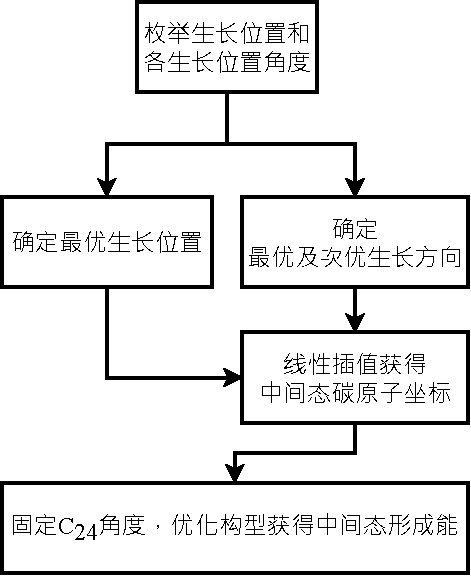
\includegraphics[width=0.4\textwidth]{pic/GO_calculateFlow.pdf}
        }
        \subfloat[]{
            \label{fig:GO_relativeAngle}
            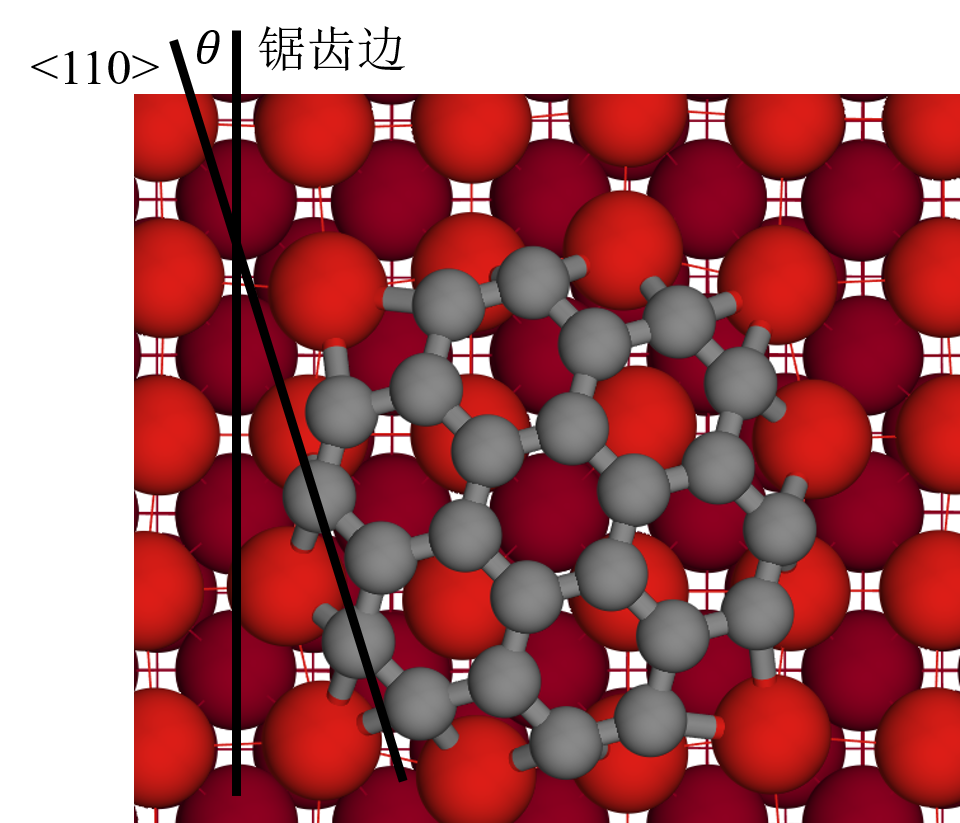
\includegraphics[width=0.4\textwidth]{pic/GO_relativeAngle.png}
        }
        \caption{计算流程图以及$\CCluster{24}$团簇生长角度标识示意图。(a)计算流程图;(b)$\CCluster{24}$团簇在铜衬底上的生长相对角度标识,其中,碳原子为灰色,铜原子为红色,不同层的铜原子以不同亮度进行区分。}
        \label{fig:GO_calculateFlow_relativeAngle}
    \end{figure}

    \subsection{石墨烯在平坦铜表面的生长晶向}
        我们首先研究石墨烯$\CCluster{24}$团簇在平坦的铜衬底表面的优先生长晶向。如图\ref{fig:GO_001_15_structure}所示,在铜(001)晶面,我们的计算发现当$\CCluster{24}$团簇中央的空洞位于铜衬底表面的面心立方(fcc)位(图\ref{fig:GO_001_15_structure_top}),同时生长角度位15\si{\degree}时,形成能最低。同时,计算获得的$\CCluster{24}$团簇在铜(001)表面的次优生长方向为0\si{\degree},与先前的文献符合\citing{RN692-2015}。从原子结构上看,石墨烯$\CCluster{24}$团簇边缘的碳原子与衬底表面的铜原子具有较强的相互作用。边缘碳原子与衬底表面铜原子的成键使得$\CCluster{24}$团簇的中央拱起,同时也使得$\CCluster{24}$团簇向更多边缘成键的角度旋转,由此在铜(001)表面形成了15\si{\degree}的优先生长方向。

        \begin{figure}[htb]
            \subfloat[]{
                \label{fig:GO_001_15_structure_side}
                \begin{overpic}[width=0.4\textwidth]{pic/GO_C24_flat_001_15deg_structure_side.png}
                    \put(85,75){$(0 0 1)$}
                \end{overpic}
            }
            \subfloat[]{
                \label{fig:GO_001_15_structure_top}
                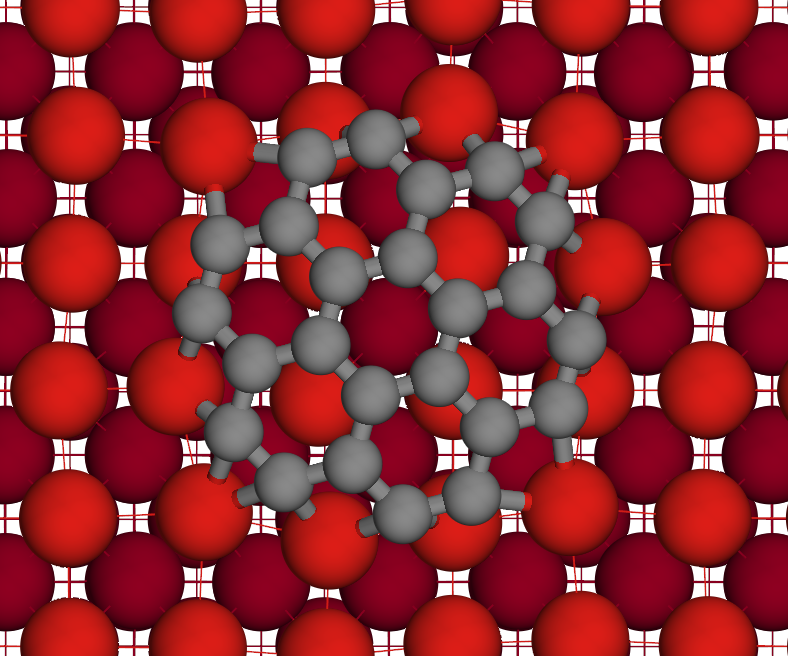
\includegraphics[width=0.4\textwidth]{pic/GO_C24_flat_001_15deg_structure_top.png}
            }

            \caption{铜(001)晶面石墨烯$\CCluster{24}$团簇的最优生长晶向(\SI{15}{\degree})及原子构型。(a)侧视图;(b)俯视图。图中,碳原子为灰色,铜原子为红色,不同层的铜原子以不同亮度进行区分。}
            \label{fig:GO_001_15_structure}
        \end{figure}

        接着,我们进一步计算了$\CCluster{24}$团簇在铜(001)表面各个角度的相对形成能,结果如图\ref{fig:GO_001_energy}所示。可以看到,$\CCluster{24}$团簇在平坦的铜(001)表面具有两个不重合的能量最小值,分别位于+15\si{\degree}和-15\si{\degree}。$\CCluster{24}$团簇在0\si{\degree}和30\si{\degree}的生长方向处于能量最高值。从能量最高的生长角度到能量最低的生长角度,$\CCluster{24}$团簇在中间态的相对能量逐渐下降。由于$\CCluster{24}$团簇在旋转至最低能态的过程中均为放热反应,因此绝大部分在成核阶段未处于最优生长方向的石墨烯晶畴会在热力学的作用下逐渐向$\pm 15$ \si{\degree} 的生长晶向靠拢。在铜(001)表面,$\pm 15$ \si{\degree} 的石墨烯$\CCluster{24}$团簇互为镜面对称,具有相同的形成能。因此在成核生长的过程中,约有一半的石墨烯畴会采取$-15$ \si{\degree}的晶向生长,而另一半则会生长为$+15$ \si{\degree}的石墨烯畴。从原子结构的角度来看,互为镜像的$\pm 15$ \si{\degree} 石墨烯畴在几何上并不重叠,由此导致了许多实验中观察到的石墨烯晶畴的非定向生长\citing{RN1062-2012}。

        \begin{figure}[htb]
            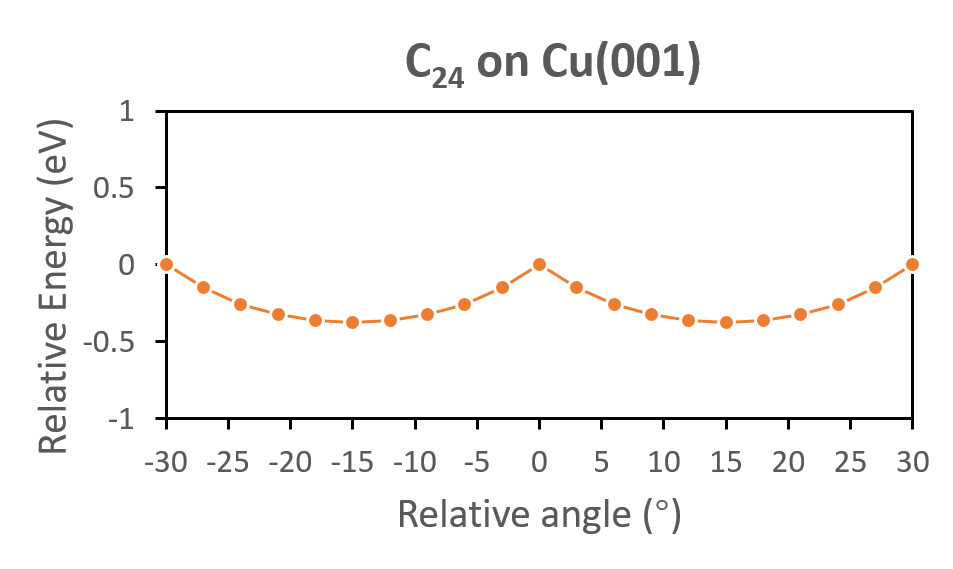
\includegraphics[width=0.8\textwidth]{pic/GO_C24_flat_001_energy.png}
            
            \caption{铜(001)晶面上不同生长角度的石墨烯$\CCluster{24}$团簇的相对形成能分布。各生长角度相对形成能的参考构型为生长角度0\si{\degree}的构型。
            }
            
            \label{fig:GO_001_energy}
        \end{figure}

        而对于铜(111)面,$\CCluster{24}$团簇在其上生长的情况与在铜(001)面类似。我们同样计算了$\CCluster{24}$团簇在平坦的铜(111)表面的最优生长位点和最优生长方向。如图\ref{fig:GO_111_structure}所示,不同于在铜(001)表面,$\CCluster{24}$团簇在平坦的铜(111)表面面上的最优生长位点为团簇中央空位垂直于铜(111)表面原子的顶端(图\ref{fig:GO_111_structure_top})。经过优化后的$\CCluster{24}$团簇的最优生长角度为$\pm 18\si{\degree}$。$\CCluster{24}$团簇边缘的碳原子同样也和铜(111)衬底表面的铜原子形成了较强的键合,使$\CCluster{24}$团簇呈现处拱起的几何形貌。$\CCluster{24}$团簇在铜(111)表面和铜(001)表面优先生长位点和方向的不同可能是来源于不同晶面指数表面对称性的变化。对于单层的铜(001)表面,其空间对称群为$P4/mmm$,为四方对称。对于单层的铜(111)表面,其空间对称群为$P6/mmm$,为六方对称。

        \begin{figure}[htb]
            \subfloat[]{
                \label{fig:GO_111_structure_side}
                \begin{overpic}[width=0.4\textwidth]{pic/GO_C24_flat_111_18deg_structure_side.png}
                    \put(80,75){$(1 1 1)$}
                \end{overpic}
            }
            \subfloat[]{
                \label{fig:GO_111_structure_top}
                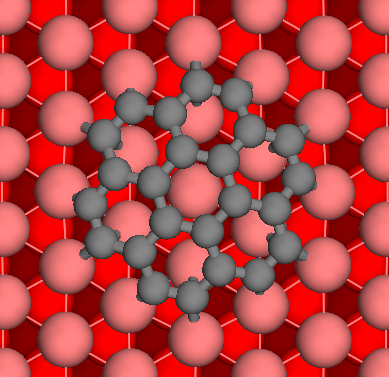
\includegraphics[width=0.4\textwidth]{pic/GO_C24_flat_111_18deg_structure_top.png}
            }

            \caption{铜(111)晶面石墨烯$\CCluster{24}$团簇的最优生长晶向(\SI{18}  {\degree})及原子构型。(a)侧视图;(b)俯视图。图中,碳原子为灰色,铜原子为红色,不同层的铜原子以不同亮度进行区分。
            }

            \label{fig:GO_111_structure}
        \end{figure}

        通过插值法,我们对平坦铜(111)表面的石墨烯$\CCluster{24}$团簇在最优生长角度之间的中间态也进行了形成能计算(图\ref{fig:GO_111_energy})。$\CCluster{24}$团簇在铜(111)上的次优生长方向为$\pm 30$\si{\degree}。由于衬底对称性的变化,在铜(111)表面,$0\si{\degree}$ 方向生长的$\CCluster{24}$团簇与$\pm 30\si{\degree}$方向生长的$\CCluster{24}$团簇并不等价。具体而言,遵循$0\si{\degree}$ 方向生长的$\CCluster{24}$团簇的锯齿(zigzag)边与铜(111)衬底的<110>方向平行,扶手椅(armchair)边与$<\bar{1}\bar{1}2>$方向平行。而遵循$\pm 30\si{\degree}$方向生长的$\CCluster{24}$团簇则相反,扶手椅(armchair)边与铜(111)衬底的<110>方向平行,锯齿(zigzag)边与$<\bar{1}\bar{1}2>$方向平行。铜$<\bar{1}\bar{1}2>$晶向的原子间距为$4.23 \si{\angstrom}$,高于铜<110>晶向中$2.56 \si{\angstrom}$的铜原子间距。从计算结果上看,$\pm 30\si{\degree}$方向生长的$\CCluster{24}$团簇的形成能比$0\si{\degree}$ 方向生长的$\CCluster{24}$团簇低大约$0.9\si{\electronvolt}$。与在平坦的铜(001)晶面上类似,$\CCluster{24}$团簇从任意生长角度到能量最低的$\pm 18 \si{\degree}$的中间态的能量逐渐下降。$\CCluster{24}$团簇在转向最优生长角度的过程均为放热反应,因此绝大部分在成核阶段未处于最优生长方向的石墨烯晶畴会在热力学的作用下逐渐向$\pm 18$ \si{\degree} 的生长晶向靠拢。从原子结构的角度来看,互为镜像的$\pm 18$ \si{\degree} 石墨烯畴在几何上并不重叠。在生长过程中的不同晶畴进行融合时仍会产生晶界。

        \begin{figure}[htb]
            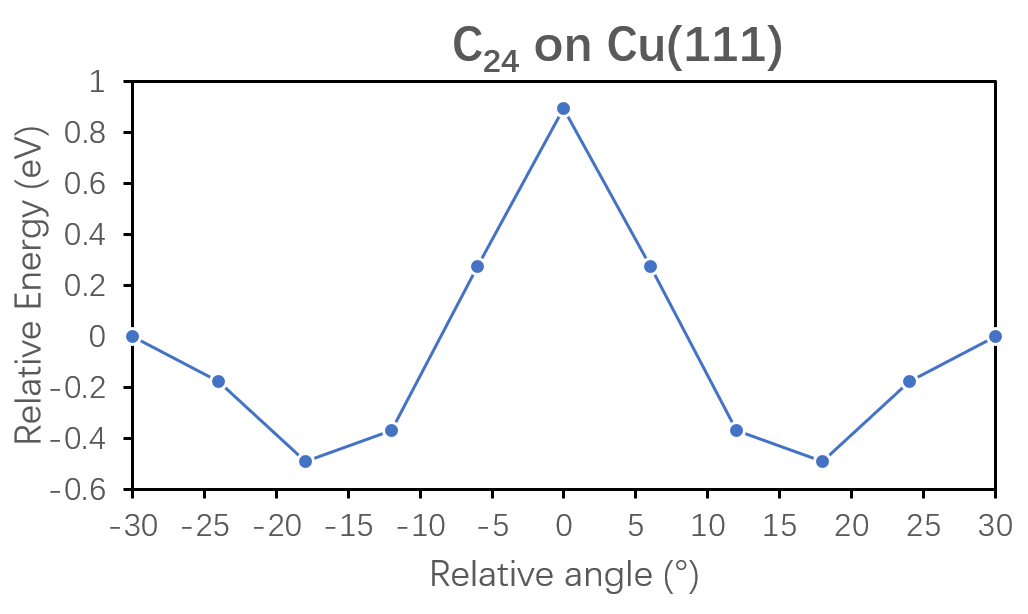
\includegraphics[width=0.8\textwidth]{pic/GO_C24_flat_111_energy.png}
            \caption{铜(111)晶面上不同生长角度的石墨烯$\CCluster{24}$团簇的相对形成能分布。各生长角度相对形成能的参考构型为生长角度$\pm 30$\si{\degree}的构型。
            }
            \label{fig:GO_111_energy}
        \end{figure}


    \subsection{石墨烯在铜表面台阶处的生长晶向}
        在本章的研究中,我们主要关注石墨烯$\CCluster{24}$团簇在晶面指数为$\rm{(11n)(n \geqslant 1)}$的铜衬底的优先生长晶向。晶面指数为$\rm{(11n)(n \geqslant 1)}$的铜表面结构可以看成由不同密度的铜(001)台面或者铜(111)台面组合而成。因此,我们可以将晶面指数为$\rm{(11n)(n \geqslant 1)}$的铜衬底分为两类\chinesecolon 一类可以看作以铜(001)台面组合而成,台阶的方向为铜<110>晶向,这类同衬底的晶面指数为$\rm{(11n)(n \geqslant 3)}$。另一类可以看作以铜(111)台面组合,台阶方向同样为铜<110>晶向,这类铜衬底的晶面指数为$\rm{(11n)(1 \leqslant n \geqslant 3)}$。而作为二者之间的铜(113)晶面,是两原子宽的铜(001)晶面加上两原宽的铜(111)晶面相对搭接而成。因此,在铜(113)表面的台阶,既可以看成是(001)台面,也可以看成是(111)台面。
        %//TODO 11n 图,包括解剖

        上一小节的计算显示,对于石墨烯$\CCluster{24}$团簇,其边缘碳原子与衬底表面铜原子的相互作用产生了$\CCluster{24}$团簇的优先生长角度。进一步的计算表明,$\CCluster{24}$团簇边缘碳原子在铜衬底表面的台阶处有相比于平坦衬底更强烈的相互作用。具体而言,如果铜(001)衬底表面有一个晶向为<110>的台阶,$\CCluster{24}$团簇在台阶边缘的形成能为$E_{\rm f}^{\rm step}=-9.02 \si{\electronvolt}$,大大高于在平坦铜(001)衬底表面的形成能$E_{\rm f}^{\rm flat}=-6.24 \si{\electronvolt}$。因此,我们可以判断,石墨烯更倾向于在铜衬底的台阶处成核。

        对于以铜(001)为台面的铜$\rm{(11n)(n \geqslant 3)}$衬底。由于石墨烯团簇与铜衬底的相互作用主要集中在团簇边缘的未饱和碳原子。并且台阶作为台面的边缘会极大的影响石墨烯团簇与铜衬底的形成能。为了不失一般性,我们以$\CCluster{24}$团簇的直径作为参考,我们建立了三个代表性的铜衬底模型。
        这三个模型分别对应于台面长度小于$\CCluster{24}$团簇直径的铜(115)晶面;台面长度大致等于$\CCluster{24}$团簇直径的铜(117)晶面;以及台面长度远大于小于$\CCluster{24}$团簇直径的$\rm (11X)(X \gg 7 )$晶面。

        对于台面长度远大于小于$\CCluster{24}$团簇直径的$\rm (11X)(X \gg 7 )$晶面(图\ref{fig:GO_C24_11X}),计算结果显示当$\CCluster{24}$团簇在台阶处成核生长时$\CCluster{24}$团簇的最优成核位置位于台阶的下方(图\ref{fig:GO_11X_structure_side}和图\ref{fig:GO_11X_structure_top}),$\CCluster{24}$团簇的中央空洞位于铜(001)台面的六方密堆(hcp)位。此时一半的$\CCluster{24}$团簇边缘与铜<110>台阶成键,另一半与铜(001)台面成键。相对于在平坦的铜(001)表面,$\CCluster{24}$团簇在铜(11X)表面的两个不重叠的最优生长角度,由于台阶的作用产生了劈裂和偏移,出现了最优生长角度和次优生长角度。

        %figure 11X
        \begin{figure}[!htb]
            \centering
            \subfloat[]{
                \label{fig:GO_11X_structure_side}
                \begin{overpic}[width=0.4\textwidth,trim={40 0 40 0},clip]{pic/GO_11X_structure_side.png}
                    \put(85,60){$\rm (1 1 X)$}
                \end{overpic}
            }
            \subfloat[]{
                \label{fig:GO_11X_structure_top}
                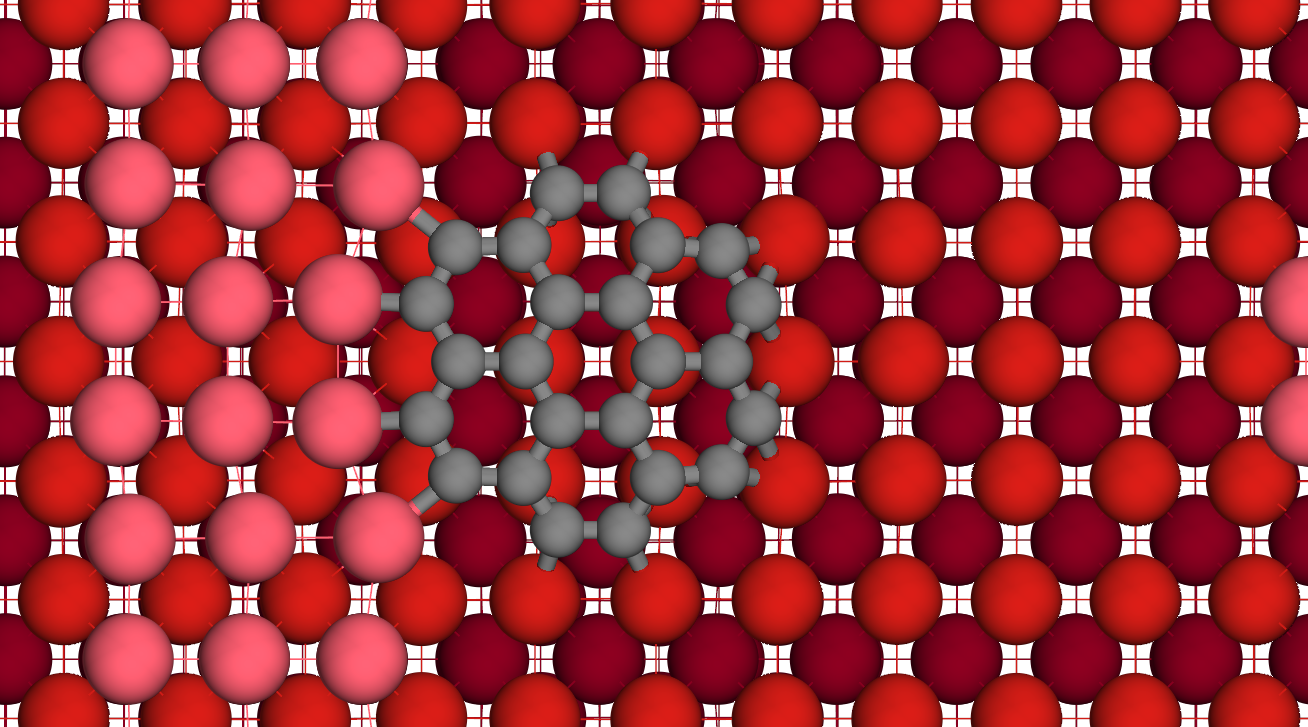
\includegraphics[width=0.4\textwidth,trim={60 20 150 20},clip]{pic/GO_11X_structure_top.png}
            }\\[-0.5ex]
            \subfloat[]{
                \label{fig:GO_11X_structure_energy}
                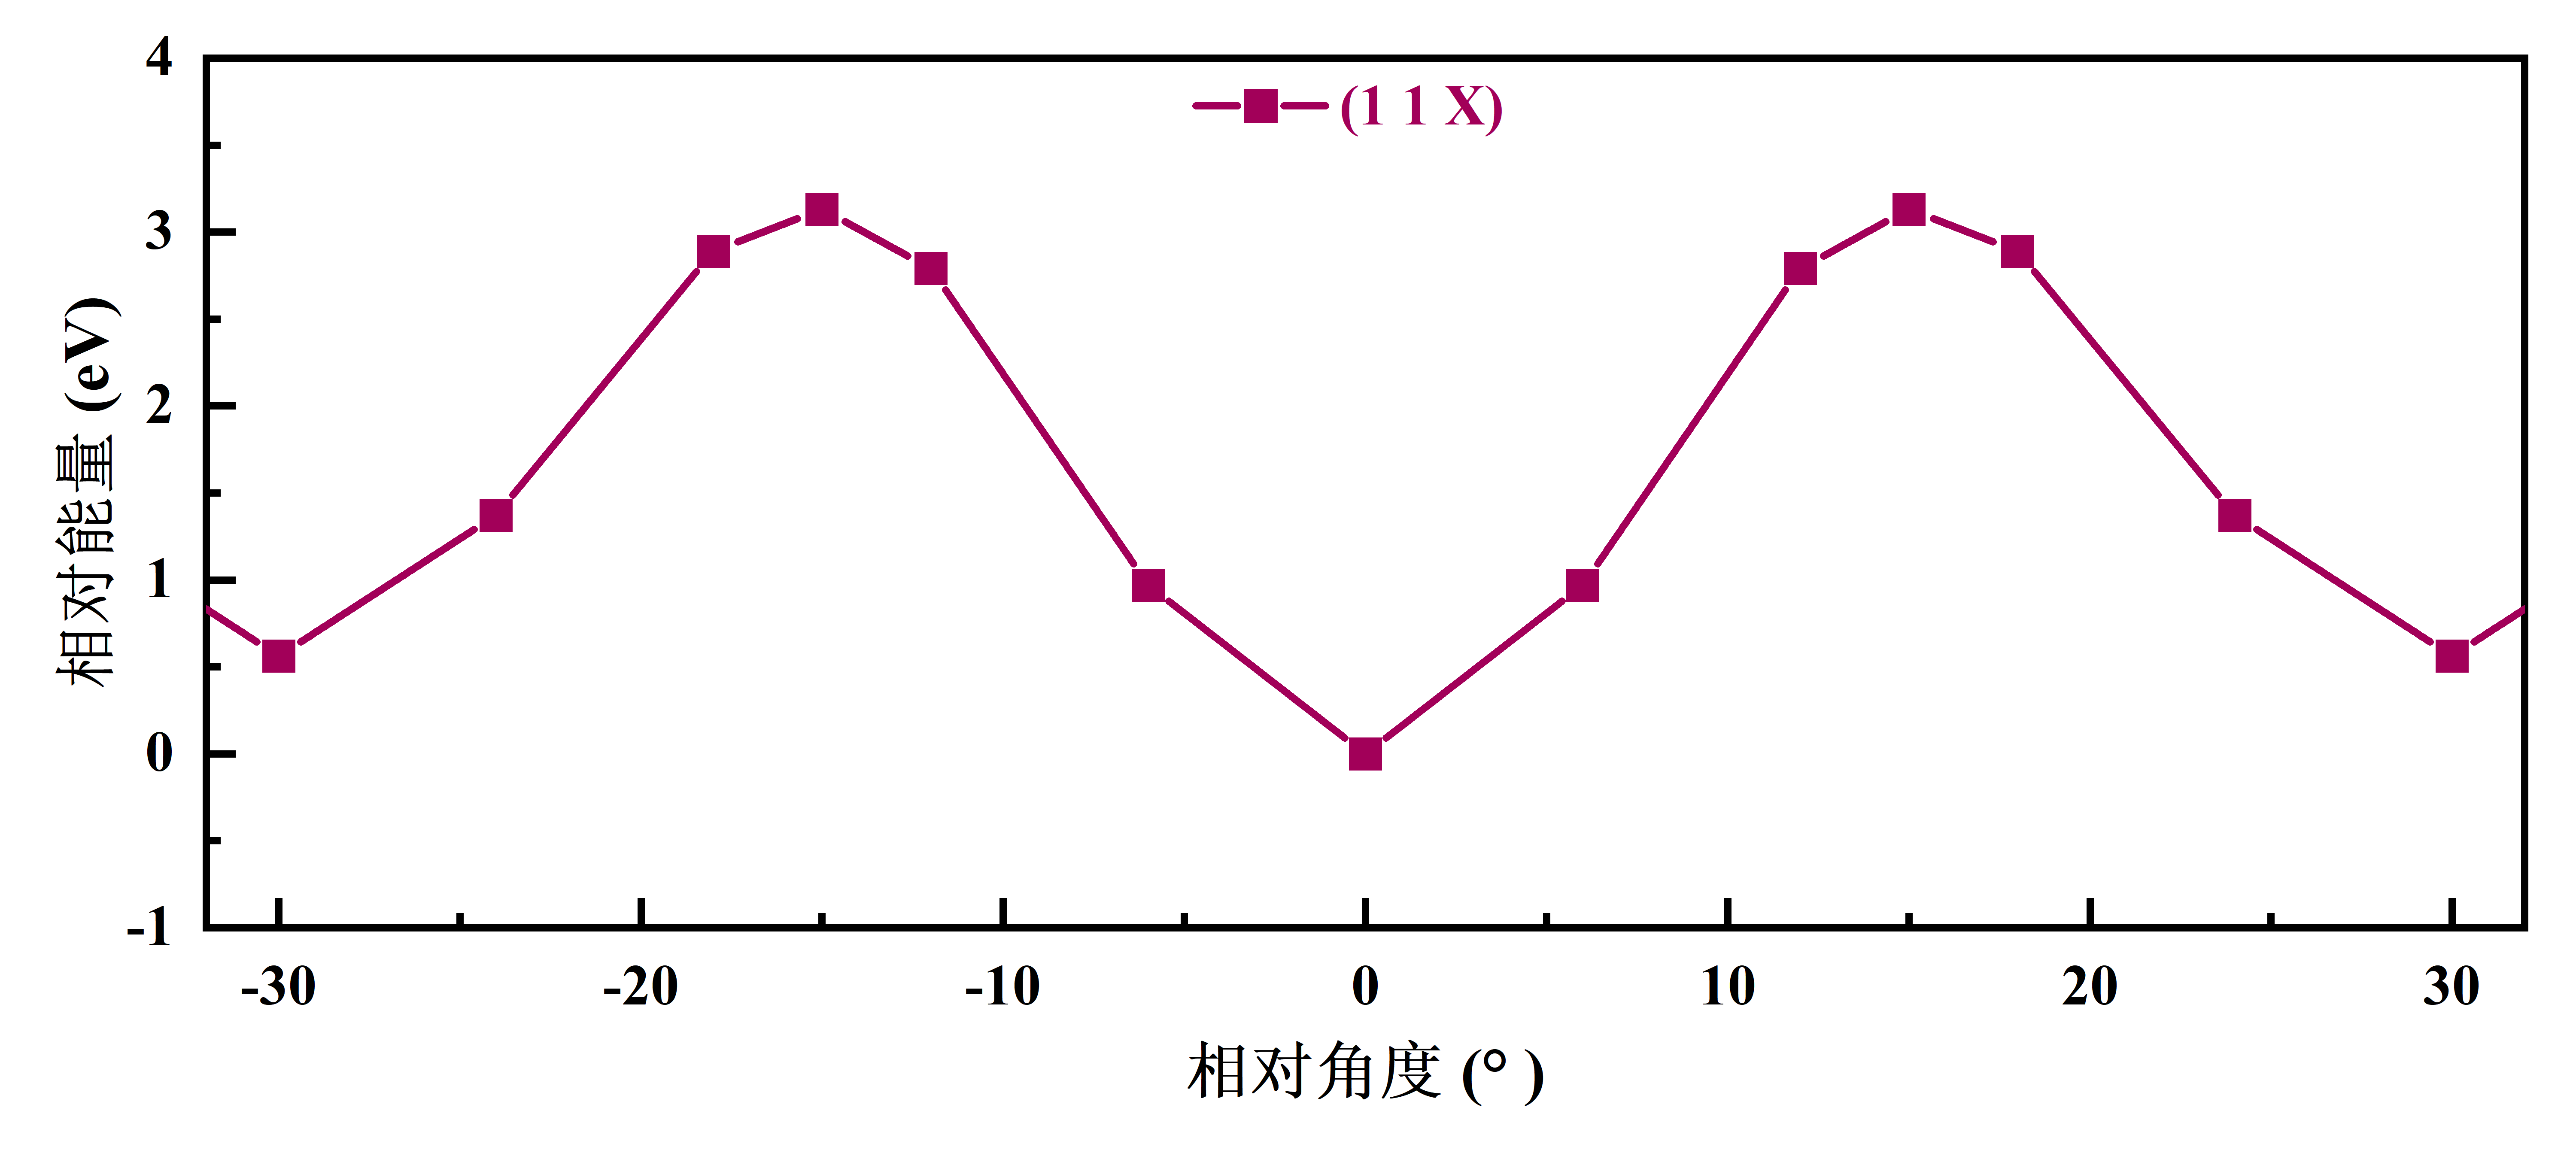
\includegraphics[width=0.8\textwidth]{pic/GO_C24_11X_energy.png}
            }
            \caption{铜(11X)晶面上石墨烯$\CCluster{24}$团簇的最优生长晶向(\SI{0}{\degree})、原子构型以及各生长角度能量分布图。(a)最优生长角度原子构型侧视图;(b)最优生长角度原子构型俯视图;(c)各生长角度能量分布。图中,碳原子为灰色,铜原子为红色,不同层的铜原子以不同亮度进行区分。}
            \label{fig:GO_C24_11X}
        \end{figure}

        从图\ref{fig:GO_11X_structure_energy}中可以看到,$\CCluster{24}$团簇在铜(11X)表面的台阶处的最优生长角度为$0\si{\degree}$,次优生长角度为$\pm 30\si{\degree}$。最优和次优生长角度之间的能量差为$0.56 \si{\electronvolt}$。$\pm 30 \si{\degree}$和$0\si{\degree}$的生长角度之间,有约为$2.56\si{\electronvolt}$的旋转势垒。单一的最优生长角度使得$\CCluster{24}$团簇在铜(11X)衬底的台阶处展现出定向生长的趋势。较高的旋转势垒使得$\CCluster{24}$团簇在成核生长的过程中需要需要较高的温度才能从次优的$\pm 30 \si{\degree}$生长角度旋转至最优的$0 \si{\degree}$。同时,由于铜(11X)衬底的(001)台面具有高于$\CCluster{24}$团簇直径的宽度,因此石墨烯晶畴很可能在远离<001>台阶的位置成核生长。在远离<001>台阶的位置成核生长的石墨烯晶畴类似于在平坦铜(001)衬底的表面生长。此时生长的石墨烯晶畴则缺乏热力学上的定向趋势。因此在铜(11X)乃至于铜(001)表面很难实现石墨烯晶畴的定向生长。

        $\CCluster{24}$团簇在铜(117)以及(115)晶面的台阶处的生长情况与铜(11X)表面相似(图\ref{fig:GO_C24_117_115})。在铜(117)晶面上,由于(001)台面的宽度与$\CCluster{24}$团簇的直径相近,$\CCluster{24}$团簇的一边与第一层台阶下边缘成键,另一层与第二层台阶的上边缘成键(图\ref{fig:GO_117_structure_side}和图\ref{fig:GO_117_structure_top})。$\CCluster{24}$团簇在铜(117)表面的最优生长位置同样也为铜(001)台面的六方密堆(hcp)位。而对于铜(115)晶面台阶处的$\CCluster{24}$团簇生长,由于铜(115)晶面上的铜(001)台面宽度仅有2原子宽,短于$\CCluster{24}$团簇的直径,所以$\CCluster{24}$团簇无法与第一层台阶的下边缘成键(图\ref{fig:GO_115_structure_side}和图\ref{fig:GO_115_structure_top})。导致在铜(115)晶面上,$\CCluster{24}$团簇的一边与第二层的台面成键,另一边与第三层台阶的上边缘成键。与第二层台阶具有较强相互作用的则是位于$\CCluster{24}$团簇中部的边缘原子。同时,由于$\CCluster{24}$团簇在(115)晶面上的生长需要横跨两层台阶,其最优生长位点相对于(11X)以及(115)晶面也有所变化。正对$\CCluster{24}$团簇中央空位的衬底位点由在(001)台面上的六方密堆(hcp)位移动至面心立方(fcc)位。

        %figure 117 115
        \begin{figure}[!htb]
            \subfloat[]{
                \label{fig:GO_117_structure_side}
                \begin{overpic}[width=0.4\textwidth,trim={60 40 40 0},clip]{pic/GO_117_structure_side.png}
                    \put(85,53){$(1 1 7)$}
                \end{overpic}
            }
            \subfloat[]{
                \label{fig:GO_117_structure_top}
                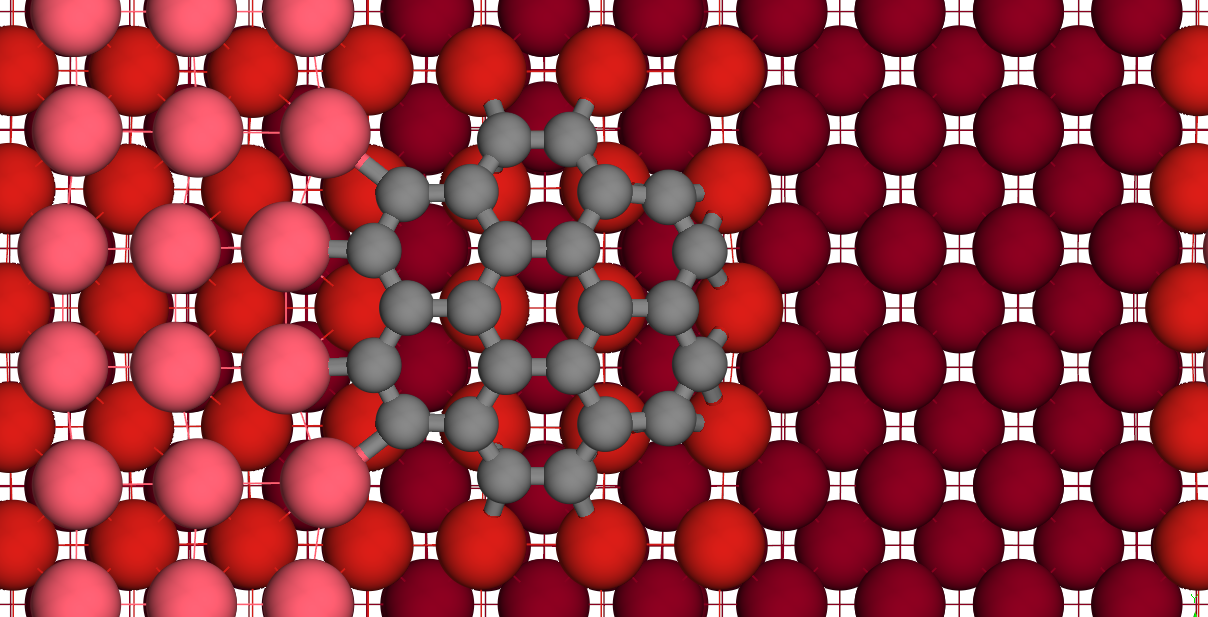
\includegraphics[width=0.4\textwidth,trim={40 0 60 0},clip]{pic/GO_117_structure_top.png}
            }\\[-1ex]
            \subfloat[]{
                \label{fig:GO_115_structure_side}
                \begin{overpic}[width=0.4\textwidth,trim={60 80 40 10},clip]{pic/GO_115_structure_side.png}
                    \put(85,53){$(1 1 5)$}
                \end{overpic}
            }
            \subfloat[]{
                \label{fig:GO_115_structure_top}
                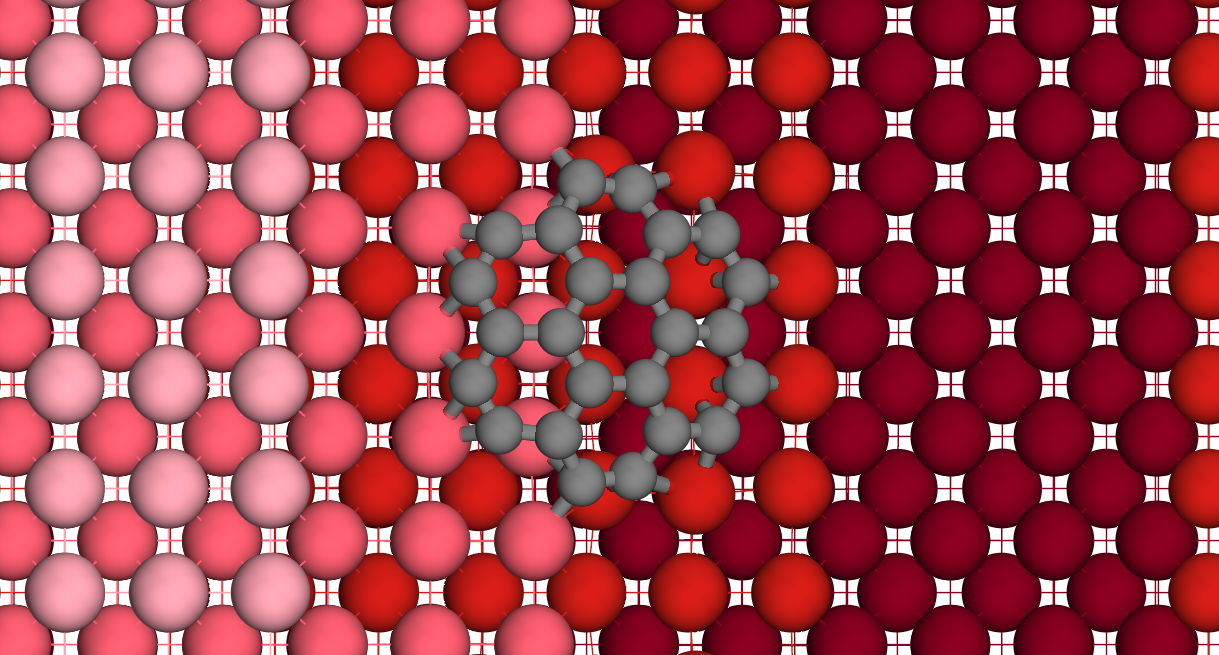
\includegraphics[width=0.4\textwidth,trim={60 20 120 40},clip]{pic/GO_115_structure_top.png}
            }\\[-0.5ex]
            \subfloat[]{
                \label{fig:GO_C24_117_115_energy}
                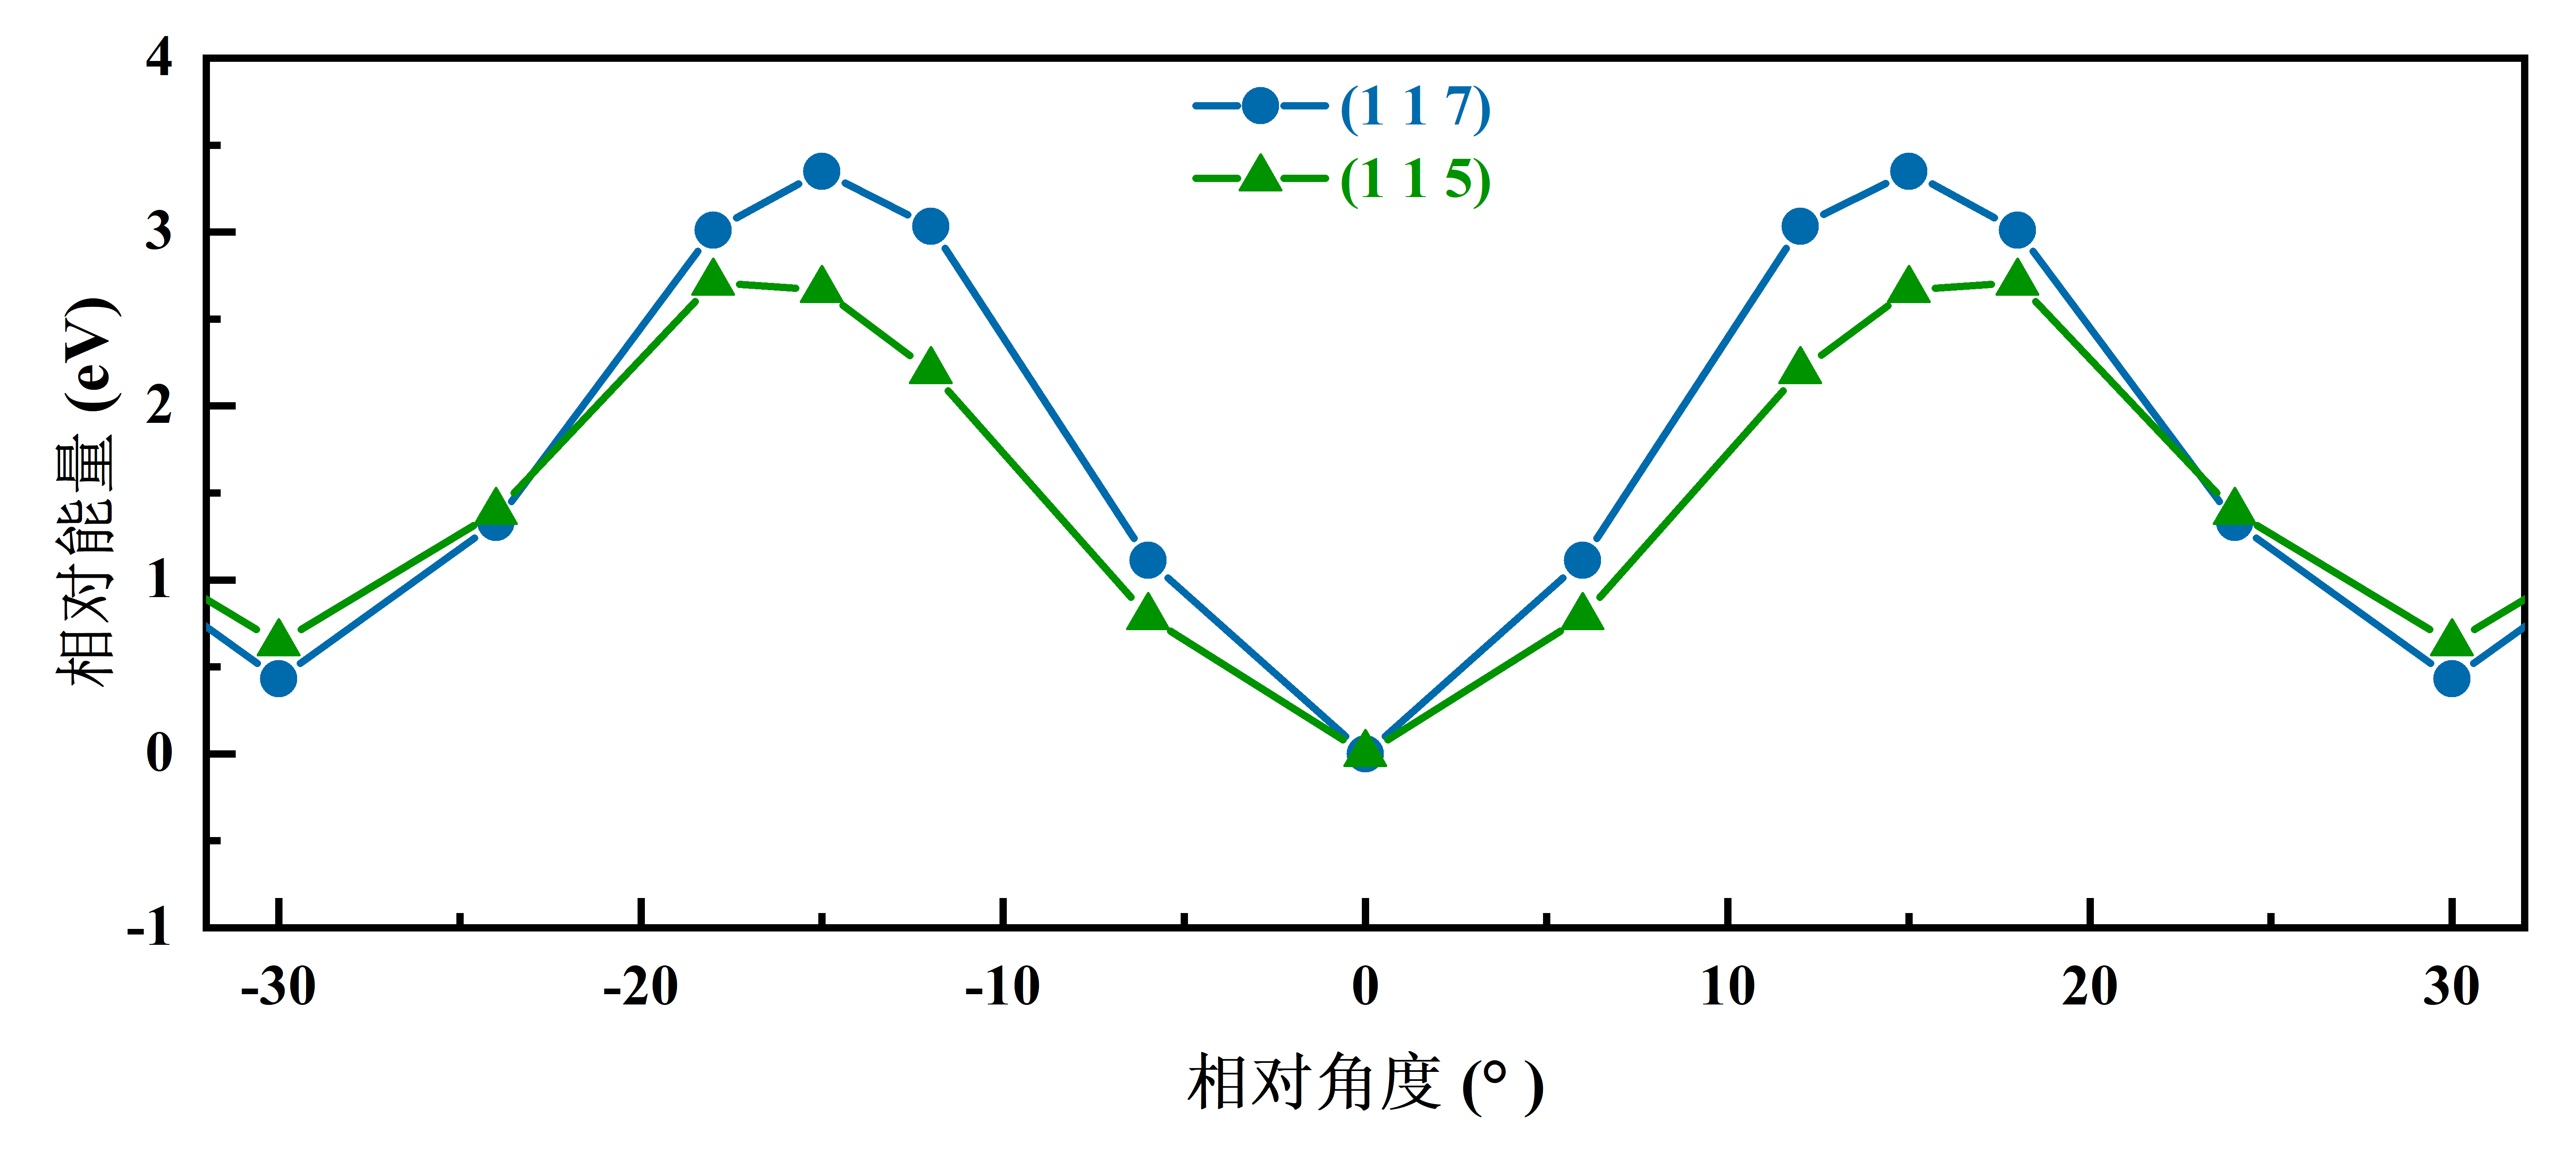
\includegraphics[width=0.8\textwidth]{pic/GO_C24_117_115_energy.png}
            }
            \caption{铜(117)与(115)晶面上石墨烯$\CCluster{24}$团簇的最优生长晶向(\SI{0}{\degree})、原子构型以及各生长角度能量分布图。(a)(117)晶面最优生长角度原子构型侧视图;(b)(117)晶面最优生长角度原子构型俯视图;(c)(115)晶面最优生长角度原子构型侧视图;(d)(115)晶面最优生长角度原子构型俯视图;(e)(117)与(115)晶面上$\CCluster{24}$团簇各生长角度能量分布。图中,碳原子为灰色,铜原子为红色,不同层的铜原子以不同亮度进行区分。}
            \label{fig:GO_C24_117_115}
        \end{figure}

        从能量的角度上看(图\ref{fig:GO_C24_117_115_energy}),$\CCluster{24}$团簇在铜(117)以及(115)晶面的上的最优生长角度均为$0 \si{\degree}$,次优生长角度位$\pm 30 \si{\degree}$,与铜(11X)晶面台阶处一致。在铜(117)晶面上,$\CCluster{24}$团簇在次优生长角度和最优生长角度之间的能量差为$0.43\si{\electronvolt}$。这个能量差低于$\CCluster{24}$团簇在铜(11X)晶面台阶边缘的$0.56\si{\electronvolt}$次优-最优角能量差,导致在铜(117)晶面上$\CCluster{24}$团簇从次优生长角转向最优生长角的比例不及生长在(11X)晶面台阶处的$\CCluster{24}$团簇,使得铜(117)晶面上生长的石墨烯的定向性下降。同时,$\CCluster{24}$团簇从次优的$\pm 30 \si{\degree}$生长角度转向最优的$0\si{\degree}$需要克服的旋转势垒为$2.91 \si{\electronvolt}$,同样高于$\CCluster{24}$团簇在铜(11X)晶面台阶处的旋转势垒。较高的旋转势垒会导致$\CCluster{24}$团簇从次优生长角向最优生长角的转变难度上升,需要更多的能量或者更长的时间才能反应至最稳态。由于石墨烯晶畴的成核生长与石墨烯晶畴向最优生长角的转变是同时进行的,石墨烯晶畴的进一步生长会引入更多的边缘原子与衬底键合,可能会导致旋转势垒提高到无法依靠热能逾越的地步。因此较高的旋转势垒也可能会导致石墨烯晶畴的定向性下降。对于铜(115)晶面,$\CCluster{24}$团簇在次优生长角度和最优生长角度之间的能量差为$0.64\si{\electronvolt}$,高于铜(117)晶面以及铜(11X)晶面。同时对于$\CCluster{24}$团簇,在铜(115)晶面上成核生长时,在热力学的作用下从次优生长角度旋转至最优生长角度所需要跨越的旋转势垒为$2.07 \si{\electronvolt}$,低于在铜(117)以及(11X)晶面的旋转势垒。
        
        通过以上计算,我们可以发现,虽然台面的宽度有所差距,但是对于晶面指数为$\rm{(11n)(n \geqslant 3)}$铜衬底而言,衬底表面的台阶对石墨烯晶畴的生长方向均有限制作用。其中以(115)晶面铜衬底最能够使石墨烯晶畴依照以$0 \si{\degree}$的生长角度进行定向成核生长。
        
        对于以(111)为台面的铜(112)晶面,$\CCluster{24}$团簇在其台阶处的成核生长行为与在平坦的铜(111)衬底表面有较大的不同(图\ref{fig:GO_C24_112})。在铜(112)晶面,由于台面的宽度短于$\CCluster{24}$团簇的直径,$\CCluster{24}$团簇无法直接于第一层台阶的下边缘成键。优化后的最优构型显示$\CCluster{24}$团簇在铜(112)晶面上成核生长时倾向于跨越一层铜<110>台阶(图\ref{fig:GO_112_structure_side}和图\ref{fig:GO_112_structure_top})。$\CCluster{24}$团簇的一边与第一层的铜台面成键,另一边与第二层的铜台阶的上表面成键。在台阶的作用下,$\CCluster{24}$团簇在铜(112)台面上的最优生长方向为$0\si{\degree}$。如图\ref{fig:GO_112_structure_energy}所示,台阶对于$\CCluster{24}$晶畴边缘碳原子较强的相互作用同样使得(111)台面上两个不重叠的最优生长角度($\pm 18 \si{\degree}$)劈裂、偏移至$0\si{\degree}$和$\pm 30 \si{\degree}$。对于铜(112)晶面,$\CCluster{24}$团簇的最优生长角度为$0\si{\degree}$,次优生长角度为$\pm 30 \si{\degree}$。次优-最优生长角度之间的能量差为$0.33\si{\electronvolt}$,低于先前计算的以铜(001)台面为基础的台阶模型。可以判断$\CCluster{24}$团簇在铜(112)衬底上的定向性弱于铜$\rm{(11n)(n \geqslant 3)}$衬底。旋转势垒方面,在铜(112)衬底上生长的石墨烯从次优的$\pm 30 \si{\degree}$旋转至最优的$0\si{\degree}$所需要克服的势垒为$1.57 \si{\electronvolt}$,低于铜$\rm{(11n)(n \geqslant 3)}$衬底衬底。因此在铜(112)台面,石墨烯晶畴可以在更低的生长温度下从非定向生长演化为定向生长。

        %figure 112
        \begin{figure}[htb]
            \subfloat[]{
                \label{fig:GO_112_structure_side}
                \begin{overpic}[width=0.4\textwidth,trim=30 20 20 0,clip]{pic/GO_112_structure_side.png}
                    \put(85,53){$\rm (1 1 2)$}
                \end{overpic}
            }
            \subfloat[]{
                \label{fig:GO_112_structure_top}
                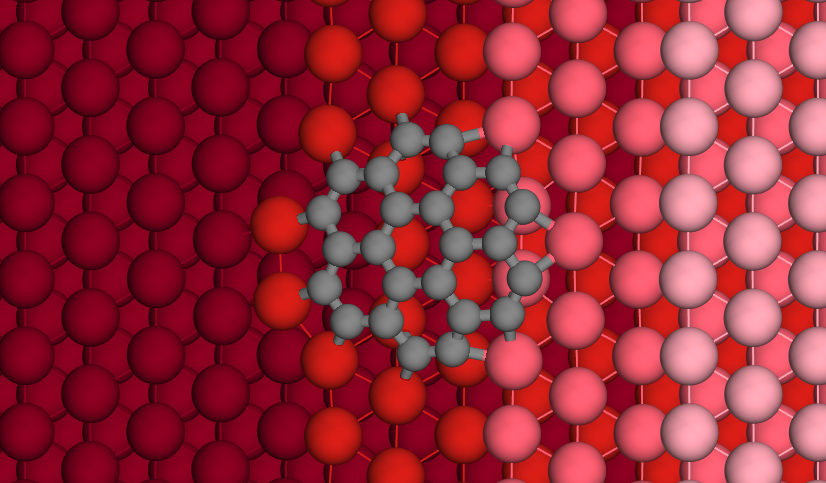
\includegraphics[width=0.4\textwidth,trim=80 40 50 40,clip]{pic/GO_112_structure_top.png}
            }\\[-0.5ex]
            \subfloat[]{
                \label{fig:GO_112_structure_energy}
                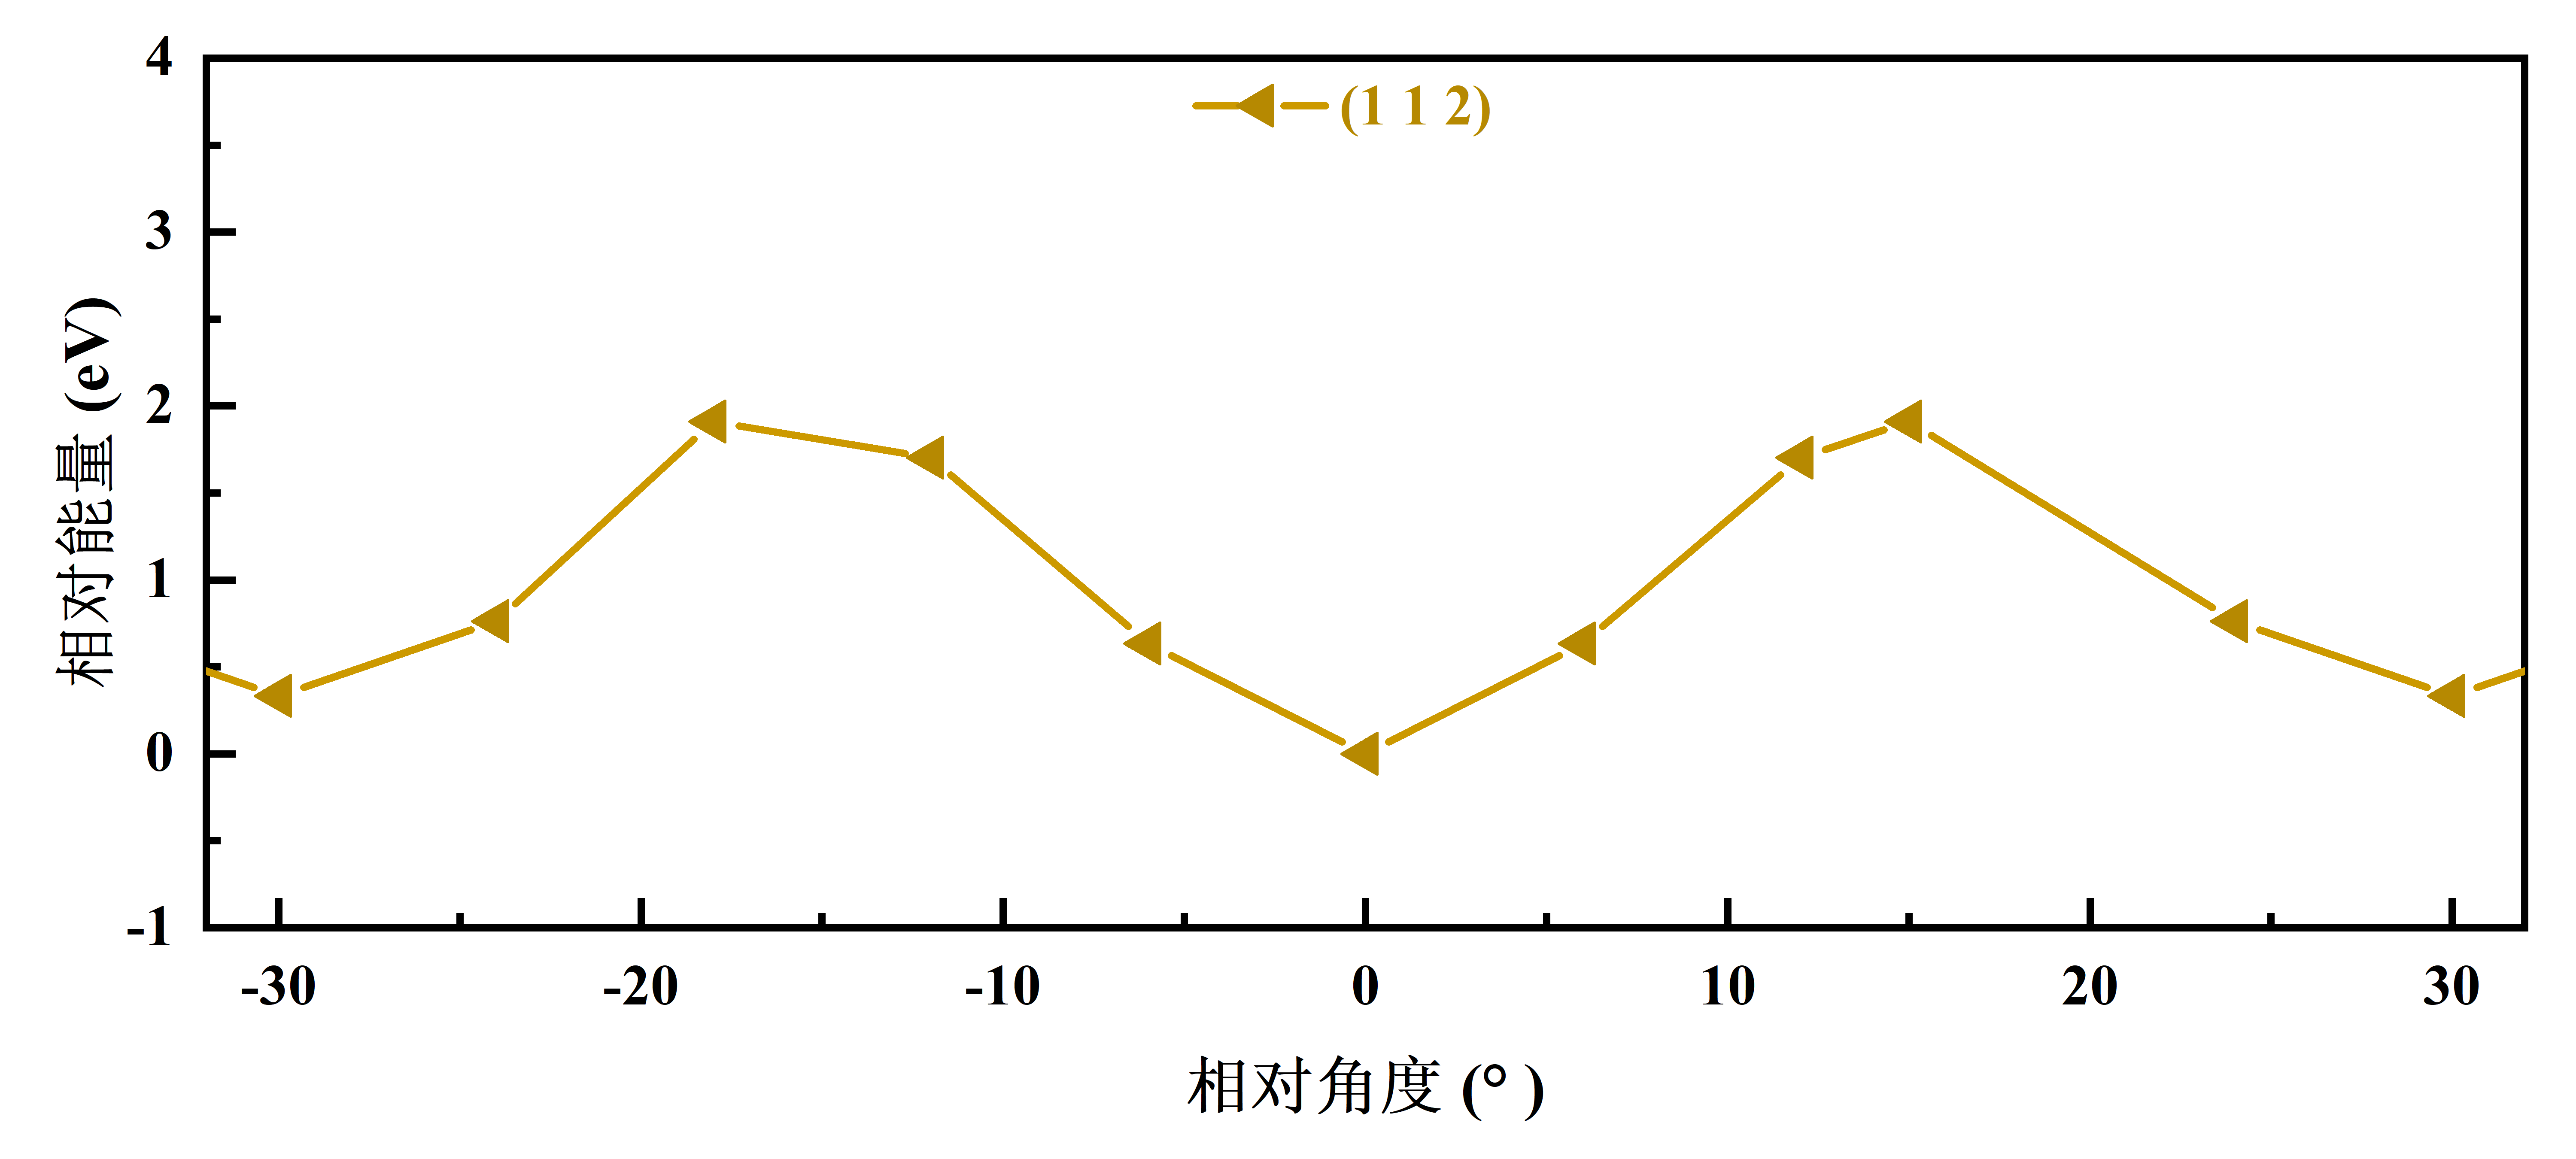
\includegraphics[width=0.8\textwidth]{pic/GO_C24_112_energy.png}
            }
            \caption{铜(112)晶面上石墨烯$\CCluster{24}$团簇的最优生长晶向(\SI{0}  {\degree})、原子构型以及各生长角度能量分布图。(a)最优生长角度原子构型侧视图;(b)最优生长角度原子构型俯视图;(c)各生长角度能量分布。图中,碳原子为灰色,铜原子为红色,不同层的铜原子以不同亮度进行区分。}
            \label{fig:GO_C24_112}
        \end{figure}

        而对于铜(113)面,(001)台面和(111)台面的相互交错不仅使得铜(113)面具有在晶面指数为$\rm{(11n)(n \geqslant 1)}$这一系列的铜衬底中拥有最高的表面能\citing{RN1063-1993},同时也对石墨烯$\CCluster{24}$团簇的定向产生了极大的影响。从图\ref{GO_C24_113}中我们可以看到,在铜(113)面上,$\CCluster{24}$团簇的最优生长构型不仅横跨两个铜台面,同时团簇两边的边缘碳原子都与<110>台阶产生了强烈的相互作用。同时,$\CCluster{24}$团簇在铜(113)表面的最优生长角度也发生了变化,为几何相互不重叠的$\pm 27 \si{\degree}$。因此,类似平坦的铜(001)表面以及铜(111)表面,石墨烯团簇在铜(113)表面无法实现能量上的定向生长。

        %figure 113
        \begin{figure}[htb]
            \subfloat[]{
                \label{fig:GO_113_structure_side}
                \begin{overpic}[width=0.4\textwidth, trim=20 20 20 30,clip]{pic/GO_113_structure_side.png}
                    \put(85,45){$\rm (1 1 3)$}
                \end{overpic}
            }
            \subfloat[]{
                \label{fig:GO_113_structure_top}
                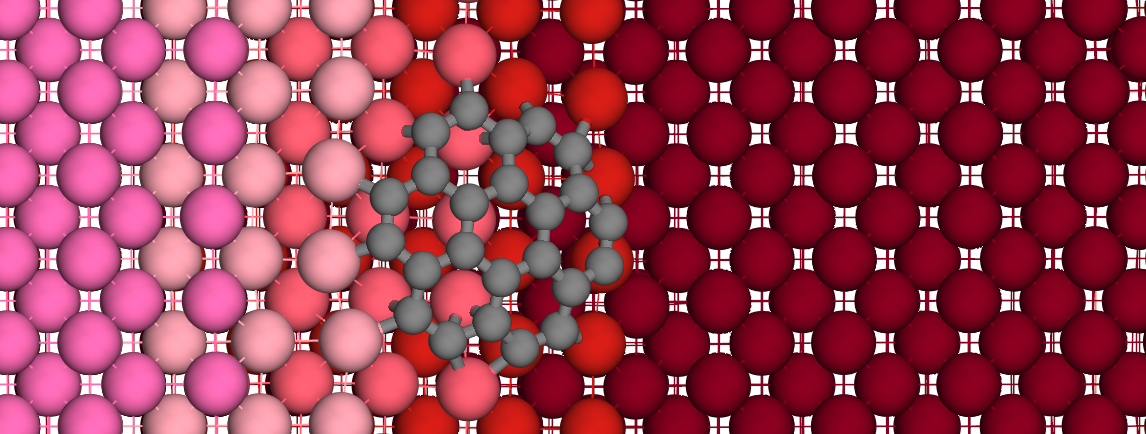
\includegraphics[width=0.4\textwidth,trim=80 0 150 0,clip]{pic/GO_113_structure_top.png}
            }\\[-0.5ex]
            \subfloat[]{
                \label{fig:GO_113_structure_energy}
                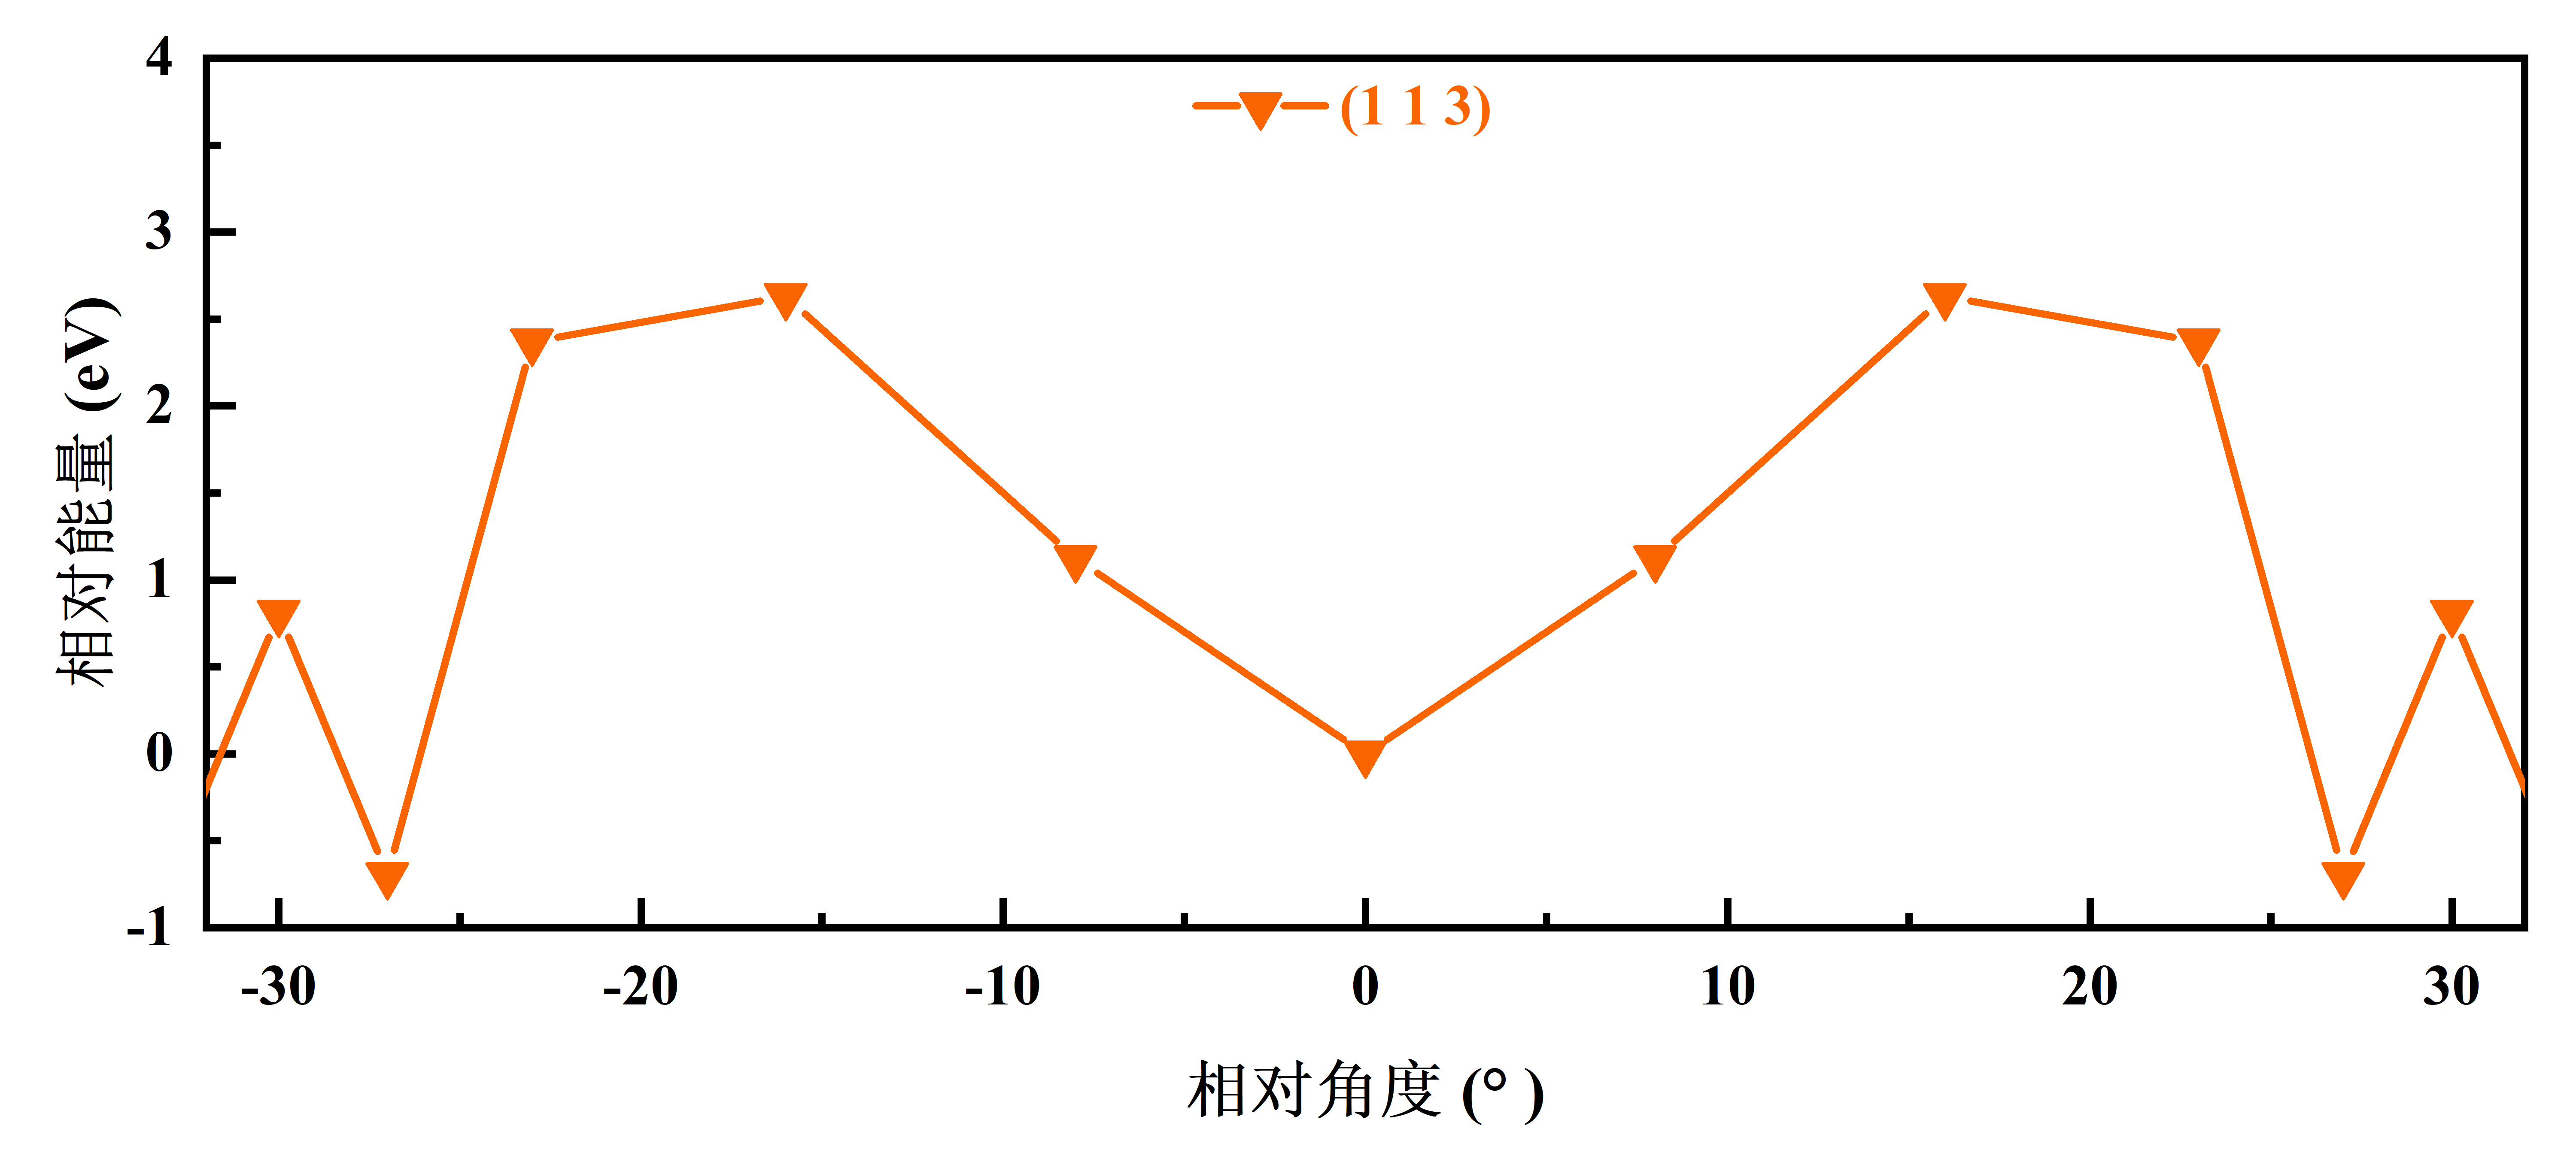
\includegraphics[width=0.8\textwidth]{pic/GO_C24_113_energy.png}
            }
            \caption{铜(113)晶面上石墨烯$\CCluster{24}$团簇的最优生长晶向($\pm 270$ \si{\degree})、原子构型以及各生长角度能量分布图。(a)最优生长角度原子构型侧视图;(b)最优生长角度原子构型俯视图;(c)各生长角度能量分布。图中,碳原子为灰色,铜原子为红色,不同层的铜原子以不同亮度进行区分。}
            \label{GO_C24_113}
        \end{figure}
        在图\ref{fig:GO_C24_energyDiff_barrier}中,我们列出了$\rm{(11n)(n \geqslant 1)}$这一系列的铜衬底上石墨烯$\CCluster{24}$团簇的定向生长能量指标。可以看到,在能够实现$\CCluster{24}$团簇定向生长的衬底中,铜(115)晶面具有最高的最优-次优生长角度能量差值,为$0.64 \si{\electronvolt}$。根据热力学的统计定律,我们可以计算$\CCluster{24}$团簇在热平衡状态下处于最优生长角度和次优生长角度的比例$r$\chinesecolon
        \begin{equation}
            r=e^{\frac{-\Delta E}{k_{\rm B}T}}
        \end{equation}
        其中$\Delta E$为两个态之间的能量差,$k_{\rm B}$为玻尔兹曼常数,$T$为温度。对于$\CCluster{24}$团簇在铜(115)晶面的成核生长,取温度$T$为常见的化学气相沉积生长石墨烯的温度$1300 \si{\kelvin}$,我们可以计算得出$\CCluster{24}$团簇处于处于最优生长角度和次优生长角度的比例$r\approx 0.0037$。即在热平衡状态写只有不到0.4\%的石墨烯$\CCluster{24}$团簇处于非定向生长的状态。而对于最优-次优生长角度差值较低的铜(112)晶面,同样计算可得$\CCluster{24}$团簇在其上生长的$r\approx 0.053$。相比于铜(115)面,铜(112)面的非定向石墨烯畴的比例上升了一个数量级。
        
        进一步考虑$\CCluster{24}$团簇在不同衬底表面从次优生长角度转变至最优生长角度的旋转势垒。在能够实现$\CCluster{24}$团簇定向生长的衬底中,铜(112)晶面具有最低的旋转势垒,为$1.57 \si{\electronvolt}$。铜(115)面紧随其后,为$2.03 \si{\electronvolt}$。更低的旋转势垒可以使$\CCluster{24}$团簇更快得达到热平衡的状态。

        \begin{figure}[!htb]
            \includegraphics[width=0.8\textwidth]{pic/GO_C24_energyDiff_barrier.png}
            \caption{$\CCluster{24}$团簇在不同衬底表面的次优-最优生长角度能量差(点)和旋转势垒(柱)。能够实现定向生长的衬底以黑点标识,无法实现定向生长的衬底以黑红点标识。}
            \label{fig:GO_C24_energyDiff_barrier}
        \end{figure}  

        综合考虑最优-次优能量差和旋转势垒的情况,我们发现对于$\rm{(11n)(n \geqslant 1)}$这一系列的铜衬底,由于由台阶的存在,石墨烯在能量上会倾向于在台阶的边缘定向生长。虽然铜(113)台面上不重叠的两个最优生长角度会使得石墨烯呈现出不定向生长的趋势,但是由于(113)台面非常高表面能,在实际生长过程中的占比很小。因此我们认为可以使用基于$\rm{(11n)(n \geqslant 1)}$这一系列的指数的多晶铜衬底,尤其是指数接近铜(112)晶面,对石墨烯进行定向生长,从而高效低成本的制备大面积单晶石墨烯。

\section{氧气对化学气相沉积法中石墨烯多层生长的作用}
\label{sec:石墨烯氧蚀刻穿透}
    \subsection{化学气相沉积法中石墨烯生长气氛模拟}
    \subsection{氧对多层石墨烯的穿透蚀刻机制}
    \subsection{氧对多层石墨烯的穿透生长机制}
    \subsection{氧在石墨烯表面的吸附过程}
    \subsection{氧辅助多层石墨烯蚀刻/生长模型及模式切换相图}
\section{总结}

